\chapter{Designing New Functionalities}
\label{chap:newfunctionalities}

Adding new functionalities to the toolbox is composed of two distinct steps: storing a new dataset (detailed in the next section), or implementing a new algorithm. This last step requires extending a predefined abstract class. A general overview of these abstract classes is shown in Fig. \ref{fig:classes}. Each class is then explained in the corresponding section in this chapter.

\begin{figure}
\centering
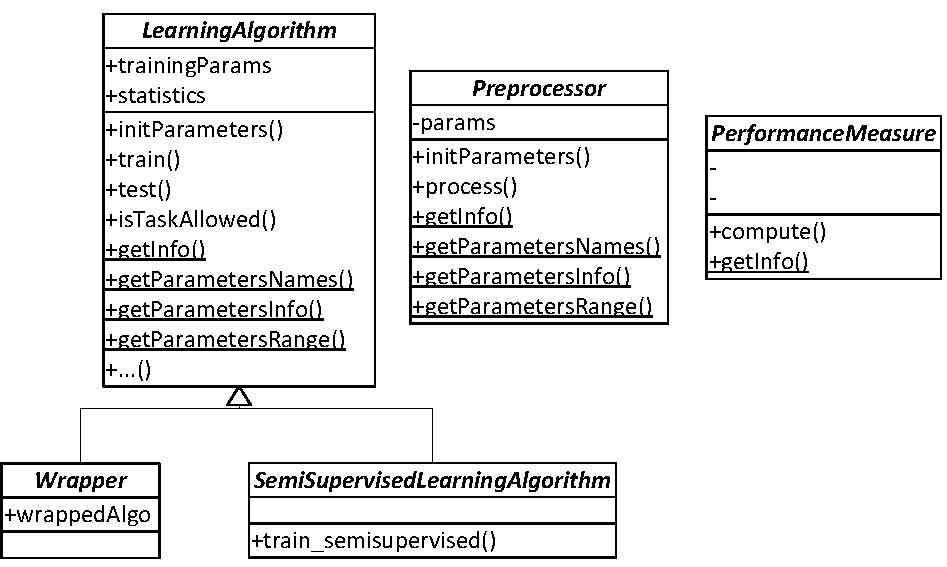
\includegraphics[scale=0.75]{./images/WrapperSchema}
\caption{Principal Abstract Classes of the Toolbox}
\label{fig:classes}
\end{figure}

\section{Storing a Dataset}
\label{sec:storingdataset}

A new dataset must be stored as a .mat file inside the ``\textit{datasets/xxx}'' folder, where \textit{xxx} is the id of the corresponding task. Each mat file must contains the following variables:

\begin{enumerate}
	\item \verb|X|: an $N \times d$ matrix of input patterns, where $N$ is the number of observations and $d$ the dimensionality of the input.
	\item \verb|Y|: an $N$-dimensional vector of corresponding output values. See Section \ref{sec:understandingtasks} for details on how each output is associated to a task.
	\item \verb|info|: a string describing the dataset.
\end{enumerate}

Matrices can be stored as dense matrices or as sparse matrices. The name of the file identifies the dataset in the program. For non-basic tasks, the following applies, as detailed in Table \ref{tab:complextasks}:

\begin{enumerate}
	\item For prediction tasks, \verb|X| is an $N$-dimensional column vector containing the samples of the time-series, while \verb|Y| is an empty matrix.
	\item For multi-label tasks, \verb|Y| is a $N \times T$ matrix, where $T$ is the number of labels. Additionally, a \verb|labels_info| variable must be present, corresponding to a $T\times1$ cell array of strings with the label descriptions.
\end{enumerate}

\section{Implementing an Algorithm}

Any algorithm should derive from the abstract class \verb|LearningAlgorithm|. This requires implementing $8$ abstract methods, $4$ of which are static. To understand this process, throughout this section we suppose we want to implement a simple K-Nearest Neighbours algorithm \cite{alpaydin2004introduction}, with the possibility of setting a given $K$.

\subsection{Setting the Training Parameters}

LearningAlgorithm defines two class properties: \verb|trainingParams| is a struct containing all the training parameters, while \verb|statistics| is a second struct where all additional information from the training process is saved. Training parameters are those that can be modified by the user when calling \verb|add\_algorithm|. They must be defined with the \verb|initParameters| method:

\begin{lstlisting}
initParameters(obj, p);
\end{lstlisting}

\noindent where \textit{p} is an InputParser object\footnote{\url{http://www.mathworks.it/it/help/matlab/ref/inputparserclass.html}}. The duty of the programmer is to fill the InputParser object with all required input parameters. The LearningAlgorithm constructor then parse its inputs, and save them in the \textit{trainingParams} struct. In our case we only have a single training parameter:

\begin{lstlisting}
classdef SimpleKNN < LearningAlgorithm
    
    properties
        knnStruct;
    end
    
    methods
        
        function obj = SimpleKNN(varargin)
            obj = obj@LearningAlgorithm(varargin);
        end
        
        function initParameters(~, p)
            p.addParamValue('K', 3, @(x) assert(mod(x,1) == x && x > 0, 'K must be an integer > 0'));
        end
        
        ...
     end
end
\end{lstlisting}

Let us analyze this. First, we define a \textit{knnStruct} that will hold the data pertaining to the training process. In the \textit{initParameters} method, we add a single parameter, and we require it to be a non-negative integer. Since we have no additional initialization requirements, the constructor of our class simply calls the base constructor of LearningAlgorithm. Example of usage of this class are:

\begin{lstlisting}
add_algorithm('K', 'K-NN', @SimpleKNN);
add_algorithm('K', 'K-NN', @SimpleKNN, 'K', 10);
\end{lstlisting}

\subsection{Training}

The next function we need to define is the one used for training a model:

\begin{lstlisting}
function obj = train(obj, Xtr, Ytr)
   obj.knnStruct = ClassificationKNN.fit(Xtr,Ytr, 'NumNeighbors', obj.trainingParams.K);                    
end
\end{lstlisting}

\verb|Xtr| and \verb|Ytr| are the input and output matrices, as defined in Section \ref{sec:understandingtasks}. In our case, we simply calls the KNN algorithm in Matlab, setting properly the number of neighbors.

In general, the algorithm's behavior may change depending on the task. The current task can be obtained by calling the \verb|getTask()| method. As an example, to check if the current task is a regression task, we can call:

\begin{lstlisting}
obj.getTask() == Tasks.R.
\end{lstlisting}

Additionally, we need to define a function describing which tasks the algorithm allows:

\begin{lstlisting}
function res = isTaskAllowed(~, ~)
   res = true;
end
\end{lstlisting}

Note that in this case we always return true, since we can use the KNN both for regression and for classification.

\subsection{Testing}

The third core method we need to define is the one used for testing. We are guaranteed that this is always called after calling the \textit{train} method. Here is an example implementation in our case:

\begin{lstlisting}
function [labels, scores] = test(obj, Xts)
   labels = predict(obj.knnStruct,Xts);
   scores = labels;
end
\end{lstlisting}

Here, \verb|Xts| is a matrix of input test patterns in the same format as the matrix for training. \verb|labels| should be an $N\times1$ vector of predictions, where $N$ is the number of rows in \verb|Xts|, with the format specified by the current task. \verb|scores| is a matrix of ``raw'' values of the algorithm, such as confidence values or probability estimates for each class. In our case, for simplicity, we set them equal to the labels.

\subsection{Class Information}

The class should define $4$ static methods describing its model and the training parameters. These methods are called when constructing the report in the \textit{help} folder. Below is a brief description of each method.

\begin{itemize}
	\item \verb|info = getInfo()| returns a string describing the algorithm.
	\item \verb|names = getParametersNames()| returns a $P\times1$ cell array of strings with the names of the training parameters.
	\item \verb|info = getParametersInfo()| returns a $P\times1$ cell array of strings with a description of each training parameter.
	\item \verb|range = getParametersRange()| returns a $P\times1$ cell array of string with the type of each training parameter (i.e. its range and possible default values).
\end{itemize}

Any algorithm inserted into the ``\textit{functionalities/algorithms}'' subfolder is automatically detected by the system.

\subsection{Implementing a Semi-Supervised Algorithm}

Implementing a semi-supervised algorithm follows the same guidelines as before. The only difference is the signature of the training method:

\begin{lstlisting}
function obj = train_semisupervised(obj, Xtr, Ytr, Xu);
\end{lstlisting}

Note that an implementation must handle the case where the additional matrix \verb|Xu| is empty.

\section{Implementing a Wrapper}

A new wrapper should derive from the abstract class \verb|Wrapper|, which itself derives from \verb|LearningAlgorithm|. The main difference is that a wrapper has an additional property, \verb|wrappedAlgo|, corresponding to an instance of its base learning algorithm.

As an example, consider part of the code for a Wrapper allowing to subsample the training dataset of a user-specified factor d:

\begin{lstlisting}
classdef Subsampler < Wrapper
	methods
		function obj = train(obj, Xtr, Ytr)
		   p = cvpartition(Ytr, 'holdout', obj.trainingParams.d);
		   obj.wrappedAlgo = obj.wrappedAlgo.setTask(obj.getTask());
		   obj.wrappedAlgo = obj.wrappedAlgo.train(Xtr(training(p), :), Ytr(training(p));
	end
end
\end{lstlisting}

The most important part in this cose is that we need to set the current task in our base algorithm, before calling its training method. In general, we may also need to access some training property of the base algorithm, or to set it to a new value (think of the \verb|ParameterSweep| wrapper). However, wrappers can nest one inside each other, and the required training parameter can in principle be at any level of the hierarchy. \verb|Wrapper| provides $2$ methods to this end: \verb|getTrainingParam| and \verb|setTrainingParam|. As an example, suppose we want to access property ``\textit{C}'' of our base algorithm. This is done as:

\begin{lstlisting}
C = obj.getTrainingParam('C');
\end{lstlisting}

\noindent Then, we increment it by one with:

\begin{lstlisting}
obj.wrappedAlgo = obj.setTrainingParam('C', C + 1);
\end{lstlisting}

\subsubsection{Evaluating an Algorithm}

A common need when designing a wrapper is that of evaluating the performance of the base algorithm using a given partition of the data. To this end, three steps are needed. First, starting from the input training matrices $X$ and $Y$ we generate an anonymous dataset:

\begin{lstlisting}
d = Dataset.generateAnonymousDataset(obj.getTask(), X, Y);
\end{lstlisting}

\noindent Successively, we generate the partitions to be used for validating. Supposing we have chosen a \verb|PartitionStrategy| ``p'', we can call:

\begin{lstlisting}
d = g.generateNPartitions(1, p);
\end{lstlisting}

\noindent Finally, we call an utility function to perform the actual test:

\begin{lstlisting}
error = eval_algo(obj.wrappedAlgo, d);
\end{lstlisting}

\section{Implementing a Preprocessor}

A preprocessor should extend the abstract class \verb|Preprocessor|. It design is very similar to that of a learning algorithm, with the following differences:

\begin{itemize}
	\item The struct of parameters is called \verb|params| instead of \verb|trainingParams|.
	\item The preprocessor needs only a single non-static method instead of \verb|train|, \verb|test|, and \verb|getAllowedTasks|. The signature of this method is:
	
\begin{lstlisting}
dataset = process(dataset);
\end{lstlisting}
	
	\noindent where \verb|dataset| is an object of class \verb|Dataset| representing the data. The output format should be in the same format.
\end{itemize}



\section{Implementing a new Performance Measure}
\label{sec:implementingperformancemeasures}

A new performance measure should derive from the base class \verb|PerformanceMeasure|, and declare two static methods:

\begin{lstlisting}
err = compute(labels, predictions);
\end{lstlisting}

\noindent where labels is an $N\times1$ vector of true labels, and predictions an $N\times1$ vector of predictions. \verb|err| should be the computed measure of error. Note that, typically, a performance measure is defined to work only on a single task (e.g., misclassification error only for classification tasks). It is the duty of the user to associate a performance measure to its required task.

\begin{lstlisting}
info = getInfo();
\end{lstlisting}

\noindent should return a string that describes the performance measure.

\section{Designing a Non-Basic Task}

Designing a non basic task requires three steps:

\begin{enumerate}
\item Defining a new task value in the class $\verb|Tasks|$.
\item Creating the corresponding folder inside ``datasets''.
\item Defining a suitable \verb|DatasetFactory| class. This must be defined inside the folder ``\textit{core/classes/DatasetFactories}'', it must be called \verb|DatasetFactoryxxx|, where \verb|xxx| is the id of the task, and it must implement a single static method:

\begin{lstlisting}
datasets = create(task, data_id, data_name, fileName, subsample, varargin);
\end{lstlisting}

\noindent where \verb|task| is the id of the task; \verb|data_id| and \verb|data_name| are th id and the name given by the user; \verb|fileName| is the name of the mat file where the dataset is stored; \verb|subsample| is the requested percentage of the dataset, in the interval $\left[0,1\right]$; and \verb|varargin| are all the additional parameters requested by the method. The output must be a cell array of \verb|Dataset| objects.
\end{enumerate}

\subsection{Designing a Partitioning Strategy}

Partitioning strategies must be extend the \verb|PartitionStrategy| class, and they must be placed inside the “\textit{core/classes/PartitionStrategies}” folder. The constructor of a partition strategy can have any number of parameters. The strategy must implement four methods:

\begin{itemize}

\item \verb|obj = partition(obj,Y)| is used to request a partition of the vector \verb|Y|. Each partition can define any number of splits of \verb|Y|, whose number must be stored in the property \verb|num_folds|.
\item \verb|ind = getTrainingIndexes(obj)| and \verb|ind = getTestIndexes(obj)| return the training and testing indexes of the current fold. The current fold can be retrieved from the property \verb| current_fold|. Indexes are $N \times 1$ vectors of logical elements, where $N$ is the dimension of the $Y$ vector of the previous method.
\item \verb|s = getFoldInformation(obj)| returns a string with information on
the current fold. This is used for printing information on the console during the simulation.
\end{itemize}

\subsection{Designing a Statistical Test}

A statistical test must extend the class \verb|StatisticalTest|. It requires the implementation of two static methods:

\begin{itemize}
\item \verb|[b, res] = check_compatibility(algorithms, datasets)| is used
to check the compatibility of the procedure with the chosen datasets
and algorithms. \verb|b| is a boolean indicating whether there is or not
compatibility. If \verb|b| is false, \verb|res| is a string describing the source of error.
\item \verb|perform_test(datasets_names, algorithms_names, errors)| performs
the test and prints the information on screen. The first two arguments are cell arrays containing the names of the datasets and of the algorithms, while the third argument is a $A \times D$ matrix of errors, where $A$ is the number of algorithms and $D$ is the number of datasets. The $ij$-th element of errors is the averaged error of the $i$-th algorithm on the $j$-th dataset.
\end{itemize}